\item En cierta computadora un programa funciona correctamente el 80\% de las veces, el 15\% interrumpe la ejecución por errores en el propio programa y el 9\% de las veces se interrumpe por errores en su entorno de trabajo, obviamente algunas veces deja de funcionar por ambas causas. Sea:
    \begin{center}
        $B=\{$La siguiente interrupción es por problemas propios del programa\}\\
        $A=$\{La siguiente interrupción es por errores en el entorno de trabajo\}\\
    \end{center}
    Calcular $P(A^c\cup B^c);P(A^c\cap B^c)$ y $P(A\cap B^c)$.
    \begin{align*}
        P(A^c\cup B^c)&=P((A\cap B)^c)\\
        &=1-P(A\cap B)\\
        &=1-P(A)-P(B)+P(A\cup B)\\
        &=1-P(A)-P(B)+1-P((A\cup B)^c)\\
        &=2-0,09-0,15-0,8\\
        &=0,96
    \end{align*}
    \begin{align*}
        P(A^c\cap B^c)&=P((A\cup B)^c)\\
        &=0,8
    \end{align*}
    \begin{align*}
        P(A\cap B^c)&=P(A-B)\\
        &=P(A-(A\cap B))\\
        &=P(A)-P(A\cap B)\\
        &=P(A)-P(A)-P(B)+P(A\cup B)\\
        &=-P(B)+1-P((A\cup B)^c)\\
        &=-0,15+1-0,8\\
        &=0,05
    \end{align*}
    Quizás una forma más intuitiva de plantear el problema sea haciendo el diagrama de Venn, para ello primero calculamos $P(A\cap B)=P(A)+P(B)-P(A\cup B)=0,09+0,15-0,2$. Entonces:
    \begin{center}
        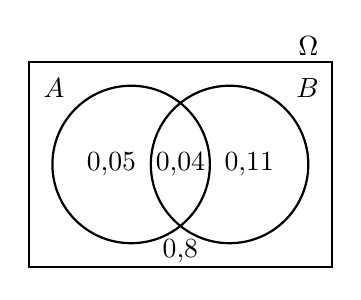
\begin{tikzpicture}[thick,
            set/.style = {circle,
                        minimum size = 2cm,
                        fill=white}]
            \draw [draw=black] (-1.3,-1.3) rectangle (2.55,1.3);
            % Set A
            \node[set,label={135:$A$}] (A) at (0,0) {};
            % Set B
            \node[set,label={45:$B$}] (B) at (1.25,0) {};
            % Circles outline
            \draw (0,0) circle(1cm);
            \draw (1.25,0) circle(1cm);
            % Set intersection label
            \node at (0.625,0) {0,04};
            \node at (-0.25,0) {0,05};
            \node at (1.5,0) {0,11};
            \node at (0.625,-1.1) {0,8};
            \node at (2.25,1.5) {$\Omega$};
        \end{tikzpicture}
    \end{center}
    Para saber $P(A^c\cup B^c)$, hay que sumar las probabilidades en naranja:
    \begin{center}
        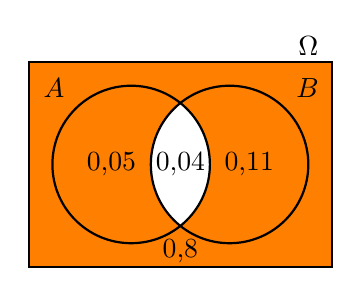
\begin{tikzpicture}[thick,
            set/.style = {circle,
                        minimum size = 2cm}]
            \fill[orange] (-1.3,-1.3) rectangle (2.55,1.3);
            \begin{scope}
                \clip (0,0) circle (1);
                \clip (1.25,0) circle (1);
                \fill[white] (1.25,0) circle (1);
            \end{scope}
            
            \draw [draw=black] (-1.3,-1.3) rectangle (2.55,1.3);
            % Set A
            \node[set,label={135:$A$}] (A) at (0,0) {};
            % Set B
            \node[set,label={45:$B$}] (B) at (1.25,0) {};
            % Circles outline
            \draw (0,0) circle(1cm);
            \draw (1.25,0) circle(1cm);
            % Set intersection label
            \node at (0.625,0) {0,04};
            \node at (-0.25,0) {0,05};
            \node at (1.5,0) {0,11};
            \node at (0.625,-1.1) {0,8};
            \node at (2.25,1.5) {$\Omega$};
        \end{tikzpicture}
    \end{center}
    Para saber $P(A^c\cap B^c)$:
    \begin{center}
        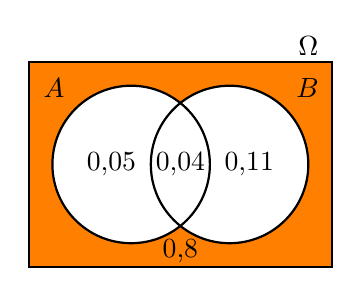
\begin{tikzpicture}[thick,
            set/.style = {circle,
                        minimum size = 2cm,
                        fill=white}]
            \fill[orange] (-1.3,-1.3) rectangle (2.55,1.3);
            \begin{scope}
                \clip (0,0) circle (1);
                \clip (1.25,0) circle (1);
                \fill[white] (-1.3,-1.3) rectangle (2.55,1.3);
            \end{scope}
            
            \draw [draw=black] (-1.3,-1.3) rectangle (2.55,1.3);
            % Set A
            \node[set,label={135:$A$}] (A) at (0,0) {};
            % Set B
            \node[set,label={45:$B$}] (B) at (1.25,0) {};
            % Circles outline
            \draw (0,0) circle(1cm);
            \draw (1.25,0) circle(1cm);
            % Set intersection label
            \node at (0.625,0) {0,04};
            \node at (-0.25,0) {0,05};
            \node at (1.5,0) {0,11};
            \node at (0.625,-1.1) {0,8};
            \node at (2.25,1.5) {$\Omega$};
        \end{tikzpicture}
    \end{center}
    Y finalmente, para $P(A\cap B^c):$
    \begin{center}
        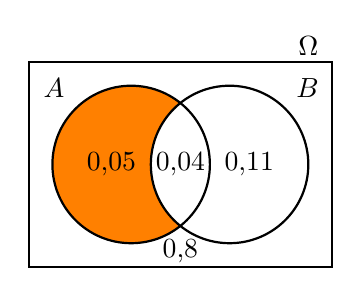
\begin{tikzpicture}[thick,
            set/.style = {circle,
                        minimum size = 2cm}]
            \fill[orange] (0,0) circle (1);
            \begin{scope}
                \clip (0,0) circle (1);
                \clip (1.25,0) circle (1);
                \fill[white] (0,0) circle (1);
            \end{scope}
            
            \draw [draw=black] (-1.3,-1.3) rectangle (2.55,1.3);
            % Set A
            \node[set,label={135:$A$}] (A) at (0,0) {};
            % Set B
            \node[set,label={45:$B$}] (B) at (1.25,0) {};
            % Circles outline
            \draw (0,0) circle(1cm);
            \draw (1.25,0) circle(1cm);
            % Set intersection label
            \node at (0.625,0) {0,04};
            \node at (-0.25,0) {0,05};
            \node at (1.5,0) {0,11};
            \node at (0.625,-1.1) {0,8};
            \node at (2.25,1.5) {$\Omega$};
        \end{tikzpicture}
    \end{center}